\chapter{Lecture ten: Function Component}
\section{Results}
The activity's primary result is a class diagram for the function component and an extension of the model component's class diagram. The secondary result of the activity is a specification of each complex operation.

Continue developing the class diagram from design of the model component.
Extend with operations realising requirements to function from the analysis of the application domain.

The purpose of the function component is to give the user interface and other system components access to the model. The function component is thus the link between the model and usage. The definition is:
\begin{center}
    \textbf{Function component:} A part of a system that implements functional requirements.
\end{center}
\begin{figure}[H]
    \centering
    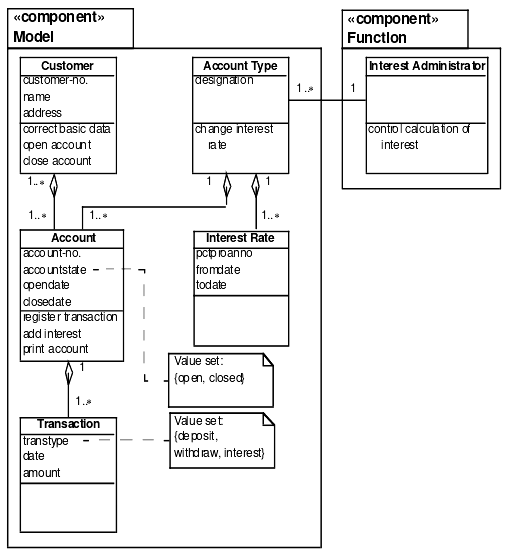
\includegraphics[width=0.5\textwidth]{figures/functioncomponentresults.png}
\end{figure}

A secondary result, the \textbf{operation specification}, is shown in the figure below.
\begin{figure}[H]
    \centering
    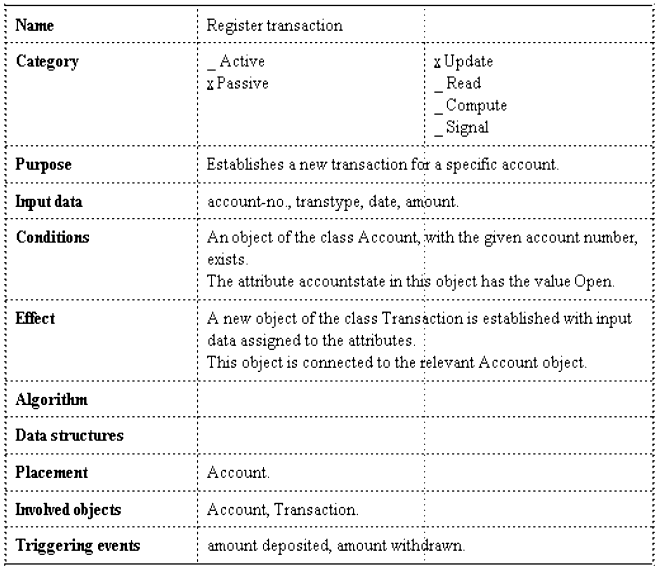
\includegraphics[width=0.7\textwidth]{figures/functioncomponentresults2.png}
\end{figure}

\section{Responsibility}
\textbf{Component:} A collection of program parts that constitutes a whole and has well-defined responsibilities.

\noindent \textbf{Responsibility of the function component:} Make the model component available as a resource to actors.

\begin{figure}[H]
    \centering
    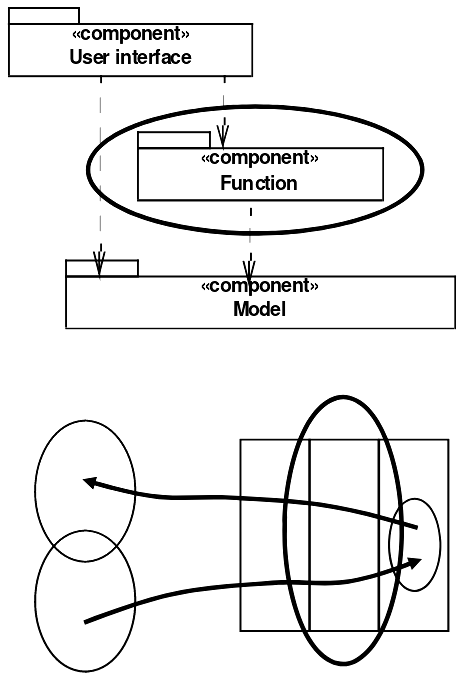
\includegraphics[width=0.3\textwidth]{figures/functioncomponentresponsibility.png}
\end{figure}

\section{Activities}

\begin{figure}[H]
    \centering
    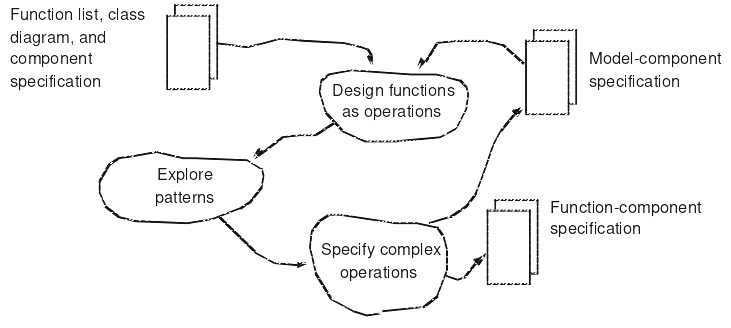
\includegraphics[width=0.7\textwidth]{figures/functioncomponentactivities.png}
\end{figure}

\section{Key concepts}

\subsection{Design functions as operations}
The four function types that we used in application-domain analysis also play a central role in designing functions as operations on classes in the model and function components. We use specific design questions for each of the four types; \textbf{update, read, compute, and signal} along with general questions for all types.

\begin{figure}[H]
    \centering
    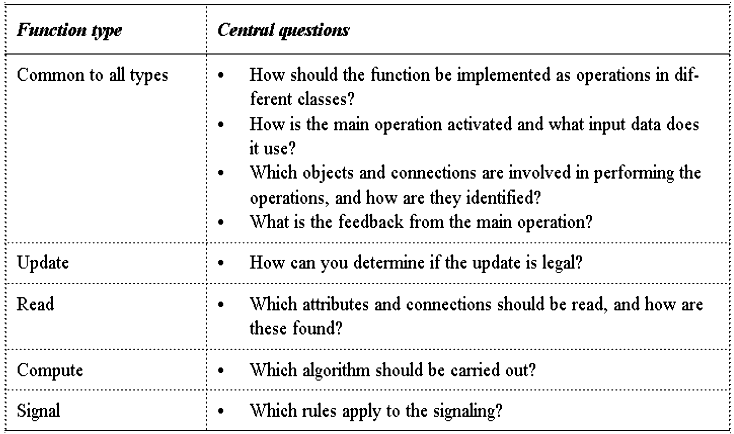
\includegraphics[width=0.7\textwidth]{figures/functioncomponentcentralquestions.png}
\end{figure}

A function will have a primary \textbf{function type}, although it may very well use attributes which are of multiple \textbf{function types}. 

\subsection{Update}
A relevant event in the problem domain must leave a trace in the model through an update function. Such a function will receive input that describes the event and may return output data to the place where the function was activated, as the figure shows.

\begin{figure}[H]
    \centering
    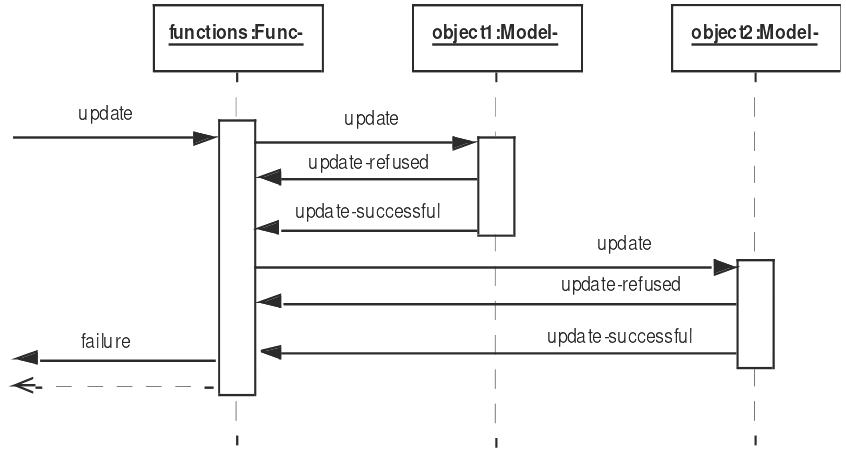
\includegraphics[width=0.5\textwidth]{figures/functioncomponentupdate.png}
\end{figure}

The relevant objects and attributes can be found by looking at the triggering events. During model-component design, one of the essential questions is how to create objects and attributes to remember events. It's this set of objects and attributes that should be updated. The input data must also be determined, afterwards the correct object should be searched for, which can either end with a set of objects or in failure.

\subsection{Read}
A read function reflects the need of a user or system to get information from the model. The system is viewed as a database. Every read requirement must be implemented by a read function, or alternatively, as a compute function.

These functions can be simple or complex, in the bank-example anything from; read balance, to read open accounts over $\$1000$ in balance. Note that update-functions might need to be called to ensure that the read-functions deliver up-to-date data.
The input to the read-function describes the wanted reading and selection of objects.

Activities are; describe the necessary operations and this can be done through precedence analysis backward from the expected output.

\begin{figure}[H]
    \centering
    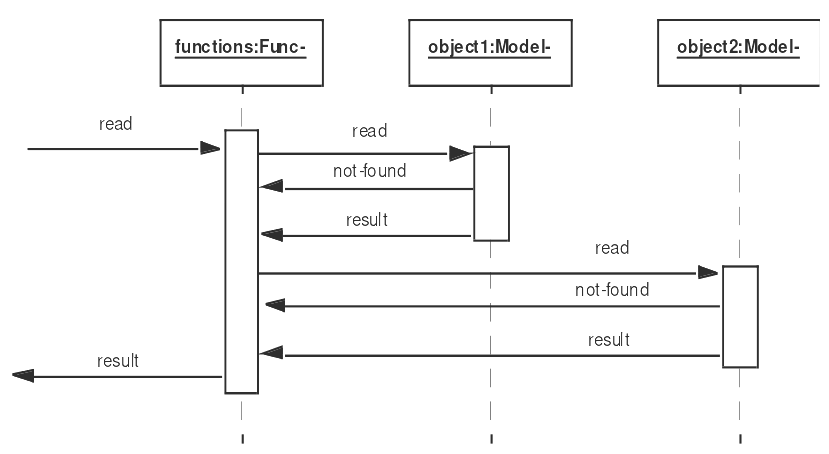
\includegraphics[width=0.5\textwidth]{figures/functioncomponentread.png}
\end{figure}

\subsection{Compute}
A compute function signifies that a user or another system needs data processing, which may involve a reading and updating of the model. The figure shows this.

Activities are; describe input and readings of the model, and describe algorithm possibly through decomposition.

\begin{figure}[H]
    \centering
    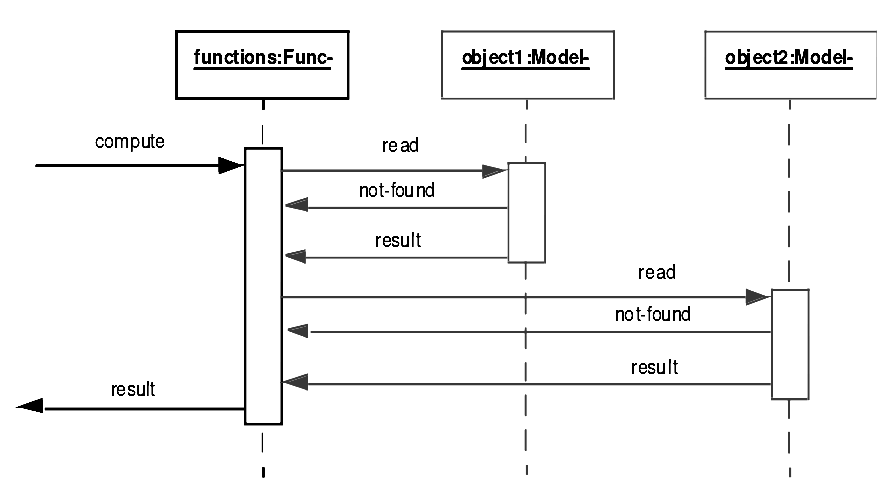
\includegraphics[width=0.5\textwidth]{figures/functioncomponentcompute.png}
\end{figure}

\subsection{Signal}
Signal functions express requirements about monitoring or control. This is applicable to actors that needs to monitor or control a part of the problem domain. The critical state is read from the model.

Typically this function has few inputs, and identifies the state transitions that might require a signal. It must be determined how to signal. This signalling might be either active or passive.


\begin{figure}[H]
    \centering
    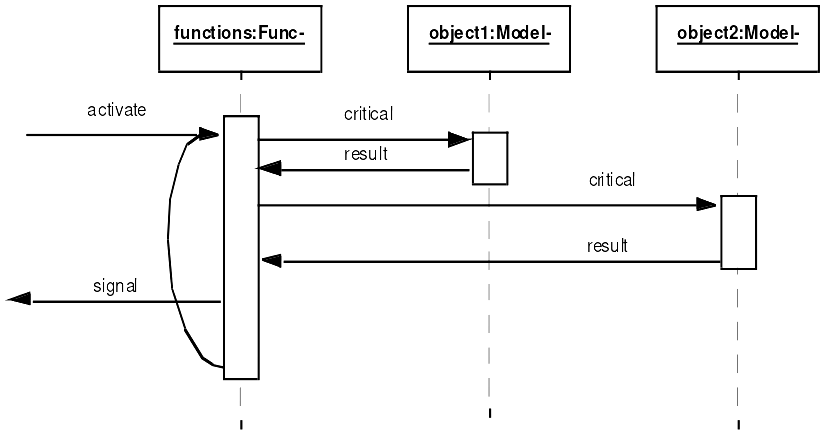
\includegraphics[width=0.5\textwidth]{figures/functioncomponentsignal.png}
\end{figure}

\section{Explore patterns}
These patterns specify how functions can be realised as a set of operations.

\subsection{Model-Class placement}
A number of operations are specified on class Account. That again is realised through several operations: transaction registration \textbf{(update)}, calculate interests \textbf{(compute)} and deposit interests \textbf{(update)}, and print account statement \textbf{(read)}.

\begin{figure}[H]
    \centering
    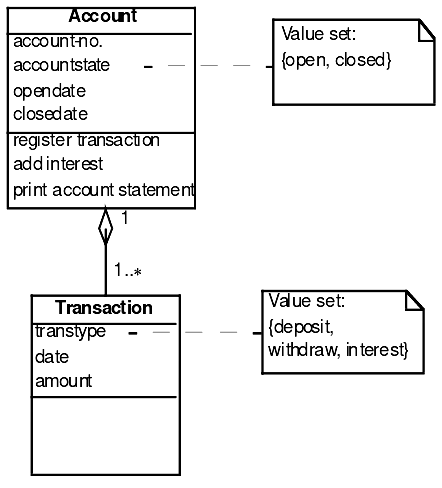
\includegraphics[width=0.3\textwidth]{figures/patternmodelclass.png}
\end{figure}

\subsection{Function-Class placement}
Some operations cannot be placed on a class in the model. Typically these are functions that operate on multiple objects. A new class is then designed in the function component. That class contains the operation that realises the function.

\begin{figure}[H]
    \centering
    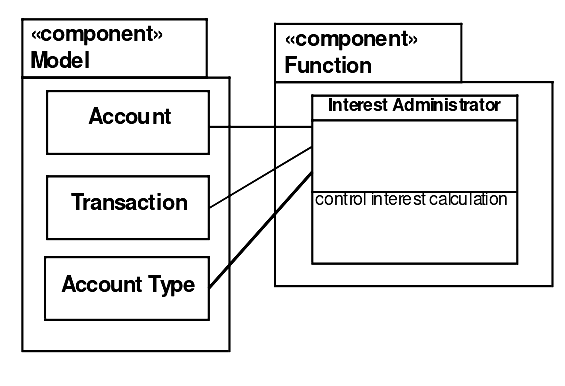
\includegraphics[width=0.35\textwidth]{figures/patternfunctionclass.png}
\end{figure}

\subsection{Strategy}
If a class has several specialisations and a function is performed differently depending on each specialisation, then the strategy pattern defines a general operation that is then described in detail in each specialisation.

\begin{figure}[H]
    \centering
    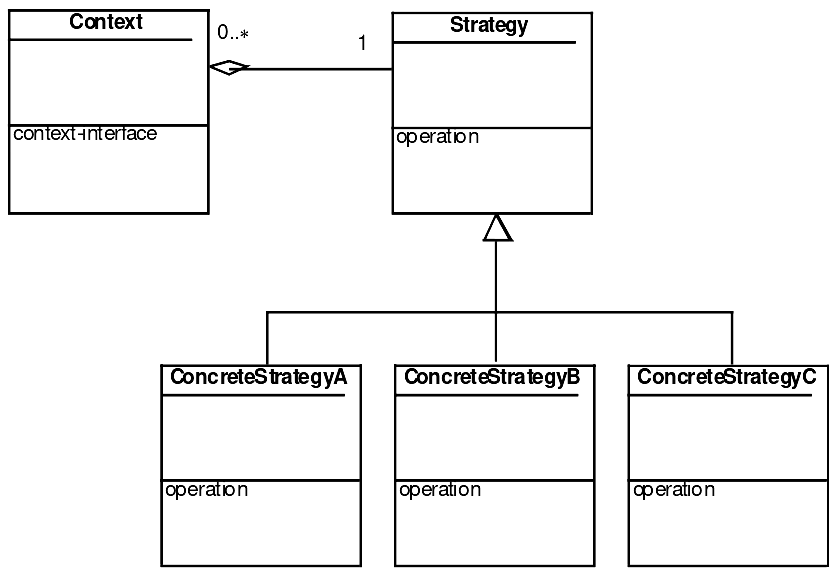
\includegraphics[width=0.6\textwidth]{figures/patternstrategy.png}
\end{figure}


\subsection{Active function}
A signal function can be active or passive. An active function can be realised in an active object. The function is then realised with its own control.

\begin{figure}[H]
    \centering
    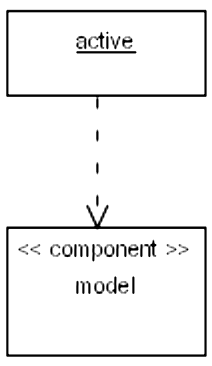
\includegraphics[width=0.15\textwidth]{figures/patternactivefunction.png}
\end{figure}

\section{Specify complex operations}
Avoid implicitly assuming the most obvious operations and merely naming other simple operations. This is especially the case for reading attributes, instead of defining these operations, you just include the attribute - the given programmer then knows that these are needed.

The textbook shows an example of an operations specification\footnote{See page 267 in \ad, for more verbose explanation}. 

\subsection{Sequence diagram}
With more complicated cases in which a function is implemented by several operations distributed over several objects, you might have to ensure that such interactions work. This can be done in a sequence diagram, which describes interactions among many objects.

\begin{figure}[H]
    \centering
    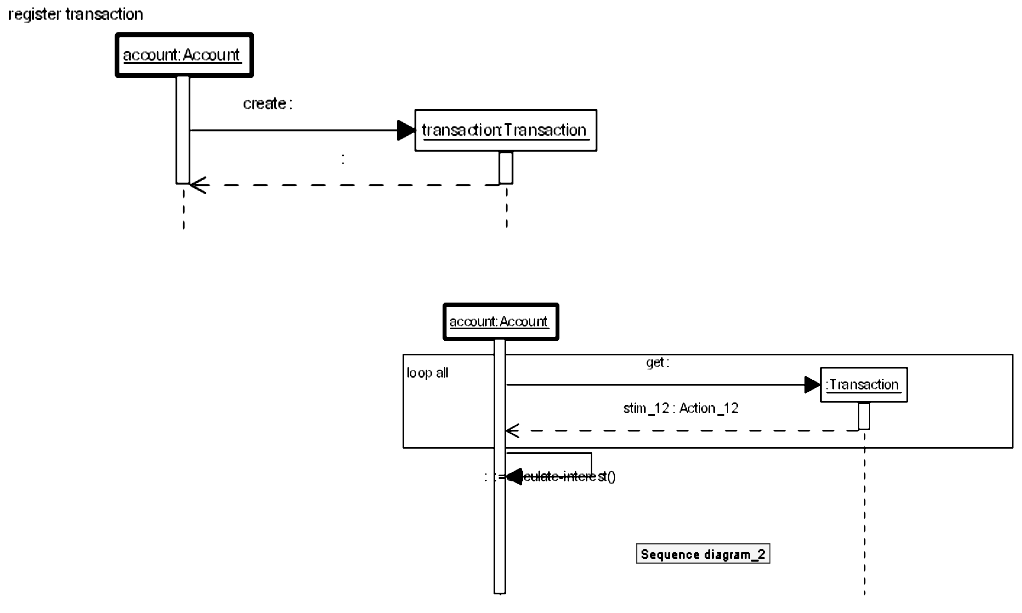
\includegraphics[width=0.8\textwidth]{figures/sequencediagram.png}
\end{figure}

\subsection{Statechart for a class}
A statechart diagram can be used to specify the relationship between an object's states and the state changes in the form of operation calls, which are received from other objects or problem-domain events. 

The figure shows a statechart diagram used in the model component to specify complex class' operations and relations between classes. 

\begin{figure}[H]
    \centering
    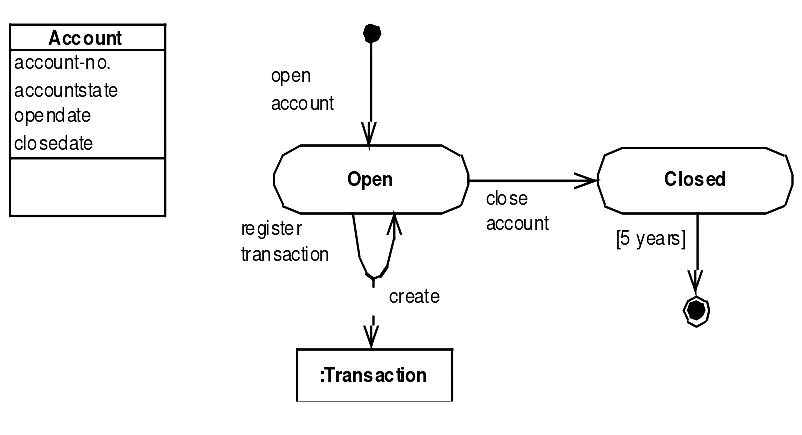
\includegraphics[width=0.65\textwidth]{figures/statechartforclass.png}
\end{figure}

\subsection{Statechart for the system's total behaviour}
During function-component design, you can use a statechart diagram to describe the system's total behaviour, especially in relation to its general states and their relations to problem-domain events. This is especially important for systems that monitor and control.

\begin{figure}[H]
    \centering
    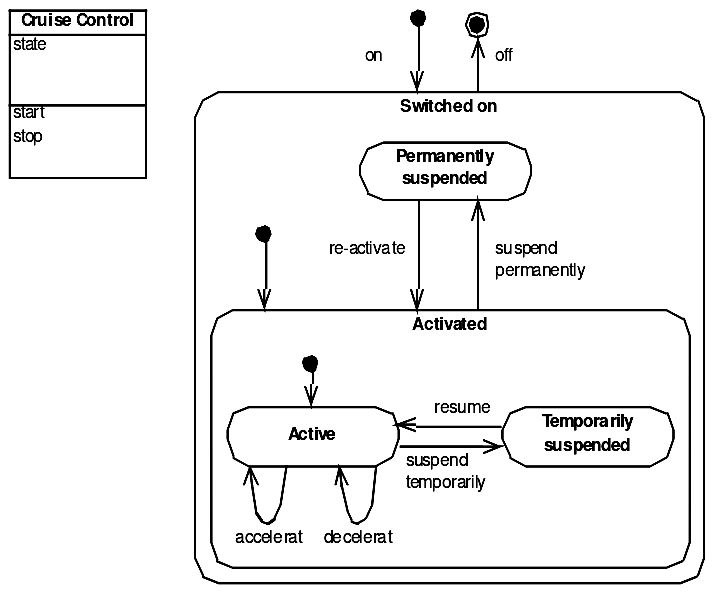
\includegraphics[width=0.6\textwidth]{figures/statechartforsystembehaviour.png}
\end{figure}

\section{Summary}

\begin{figure}[H]
    \centering
    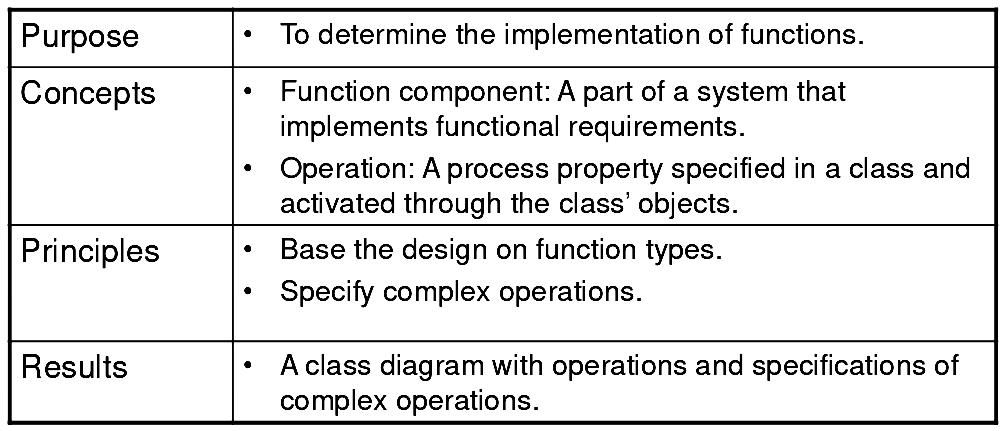
\includegraphics[width=0.7\textwidth]{figures/functioncomponentsummary.png}
\end{figure}

\section{Principles}
\subsection{Base the design on function types}
The design of individual function implementations can be based on concrete design questions that arise from the function's type.

\subsection{Specify complex operations}
The functions should be designed, not programmed. During function-component design, all essential uncertainties about the design should be eliminated, but any further detail should be avoided.